\documentclass[12pt,a4paper]{article}

\usepackage{fontawesome5}
\providecommand{\faPencilAlt}{\faIcon{pencil-alt}}

\usepackage{styles/couleurs}
\usepackage{styles/mise_en_page}
\usepackage{styles/boites}
\usepackage{styles/maths}
\usepackage{styles/figures}

\usepackage{enumitem}
\usepackage{array}
\usepackage{tabularx}
\usepackage{amsmath}
\usepackage{amssymb}
\usepackage{tikz}
\usepackage{xparse}
\usepackage{pdflscape}
\usepackage{colortbl}

\usetikzlibrary{calc,arrows.meta,positioning}

\setlist[itemize]{leftmargin=1.4em,itemsep=0.15em,topsep=0.2em}
\setlist[enumerate]{leftmargin=*,itemsep=0.22em,topsep=0.25em}

\newcommand{\lignepointillee}{\noindent\dotfill\par\vspace{0.45em}}

\newcommand{\lignesreponse}[1]{%
\begin{tcolorbox}[
enhanced,colback=white,colframe=NeutreC!40,boxrule=0.5pt,arc=1.5mm,
left=3mm,right=3mm,top=2mm,bottom=1mm,before skip=2pt,after skip=2pt]
\foreach \i in {1,...,#1}{\lignepointillee}
\end{tcolorbox}}

\newcommand{\titreseq}[1]{%
\begin{center}
{\sffamily\large\bfseries\color{SavoirC}#1}
\end{center}}

\newcommand{\grillecent}{%
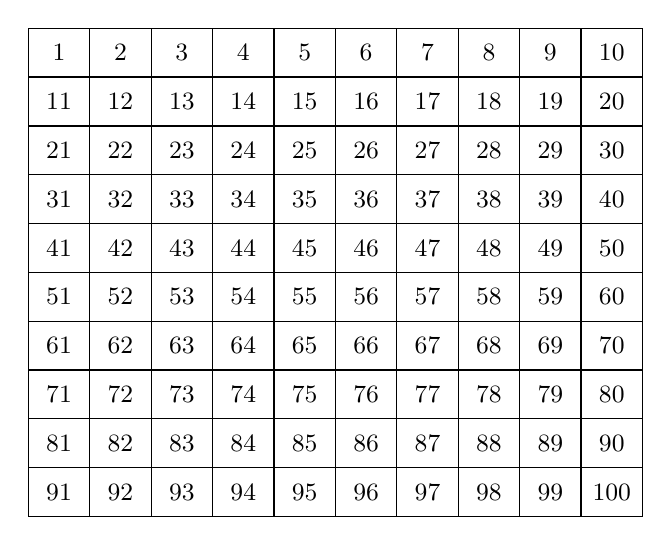
\begin{tikzpicture}[x=0.78cm,y=0.62cm]
  \foreach \n in {1,...,100}{
    \pgfmathtruncatemacro{\col}{mod(\n-1,10)}
    \pgfmathtruncatemacro{\lig}{9-floor((\n-1)/10)}
    \draw[line width=0.45pt] (\col,\lig) rectangle ++(1,1);
    \node[font=\small] at (\col+0.5,\lig+0.5) {\n};
  }
\end{tikzpicture}}

\begin{document}

\titreseq{Activité 1 -- L'atelier du menuisier}

\remarque{Cette activité réactive la division euclidienne et la lecture du quotient
et du reste. La calculatrice est autorisée uniquement pour vérifier les divisions.}

Pour construire une étagère complète, un menuisier utilise :

\[
\begin{array}{c|ccccc}
\text{Matériel} &
\text{planches longues} &
\text{planches courtes} &
\text{petites équerres} &
\text{grandes équerres} &
\text{vis}\\
\hline
\text{Pour une étagère} & 4 & 6 & 12 & 2 & 14
\end{array}
\]

Il dispose de :

\[
26\text{ planches longues},\quad
33\text{ planches courtes},\quad
200\text{ petites équerres},
\]
\[
20\text{ grandes équerres}
\quad\text{et}\quad
510\text{ vis}.
\]

\section*{Partie A -- Une première estimation}

Sans poser toutes les divisions, propose un nombre d'étagères
qui te semble possible. Explique ton estimation.

\lignesreponse{4}

\section*{Partie B -- Examiner chaque ressource}

Complète le tableau. Le quotient indique le nombre d'étagères que permettrait
la ressource si elle était la seule contrainte.

\renewcommand{\arraystretch}{1.55}
\begin{tabularx}{\textwidth}{
|>{\raggedright\arraybackslash}p{3.5cm}
|>{\centering\arraybackslash}p{2cm}
|>{\centering\arraybackslash}p{2cm}
|>{\centering\arraybackslash}X
|>{\centering\arraybackslash}X|}
\hline
\textbf{Ressource} & \textbf{Stock} &
\textbf{Besoin par étagère} &
\textbf{Quotient entier} & \textbf{Reste}\\
\hline
Planches longues & 26 & 4 & & \\
\hline
Planches courtes & 33 & 6 & & \\
\hline
Petites équerres & 200 & 12 & & \\
\hline
Grandes équerres & 20 & 2 & & \\
\hline
Vis & 510 & 14 & & \\
\hline
\end{tabularx}

\section*{Partie C -- Décider}

\begin{enumerate}
  \item Quelle ressource empêche de construire davantage d'étagères ?
  \item Combien d'étagères complètes peut-on construire ?
  \item Après cette construction, combien reste-t-il de chaque ressource ?
  \item Pourquoi ne faut-il pas choisir le plus grand quotient du tableau ?
\end{enumerate}

\lignesreponse{7}

\section*{Partie D -- Écrire une division euclidienne}

Choisis deux lignes du tableau et écris les égalités correspondantes
sous la forme :

\[
\text{dividende}
=
\text{diviseur}\times\text{quotient}
+
\text{reste}.
\]

\lignesreponse{4}

\begin{tcolorbox}[
  enhanced,
  colback=SavoirBg,
  colframe=SavoirC!60,
  boxrule=0.7pt,
  arc=2mm,
  title={\sffamily\bfseries Rappel},
  coltitle=SavoirC,
  fonttitle=\sffamily\bfseries
]
Dans une division euclidienne de \(a\) par \(b\), avec \(b\neq0\) :

\[
a=b\times q+r
\qquad\text{avec}\qquad
0\leq r<b.
\]

Le quotient entier donne le nombre de groupes complets ;
le reste indique ce qui n'a pas été utilisé.
\end{tcolorbox}

\end{document}
